\section{Static Timing Analysis}
Regarding the timing analysis, it has been defined a timing constraints file specifying a
target frequency of 100MHz (i.e. 10 nanoseconds clock period). Moreover, for each unconstrained path (input/output signals), it has been defined a maximum and a minimum delay as a percentage of the system clock, 20\% and 10\% respectively. The hardware module is able to reach a frequency of $133.32$MHz at 85°C, and a frequency of $132.89$MHz at 0°C. In both cases, the frequency is higher than the predetermined one ($100$MHz), and all constraints are met.

\section{Results}
The results and performances of the described hardware module will now be discussed.
\begin{figure}[!ht]
    \centering
    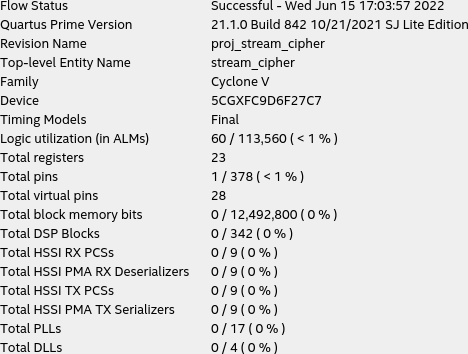
\includegraphics[width=.8\textwidth]{summary}
    \caption{Summary}
    \label{fig:summary}
\end{figure}

The usage of the hardware resources of the target FPGA is very low ($< 1\%$), which results in a waste of resources (and money). The number of total used pins is 28, as expected:
\begin{multicols}{3}
    \begin{itemize}
        \item \lstinline{rst_n}: 1 pin
        \item \lstinline{key}: 8 pins
        \item \lstinline{key_in}: 1 pin
        \item \lstinline{din}: 8 pins
        \item \lstinline{din_valid}: 1 pin
        \item \lstinline{dout}: 8 pins
        \item \lstinline{dout_valid}: 1 pin
    \end{itemize}
\end{multicols}
The clock signal (\lstinline{clk}) is the only non-virtual pin.

\clearpage
From the summary, it can be seen that the number of synthesized registers is 23. However, this number exceeds the expected one, which was 17, as deduced from the module sources. Moreover, the analysis and synthesis, as well as the netlist created by the synthesizer, show exactly 17 registers (\cref{fig:synthesizer_results_registers}), which are:
\begin{itemize}
    \item 8 for the \lstinline{cb} signal
    \item 8 for the \lstinline{dout} signal
    \item 1 for the \lstinline{dout_valid} signal
\end{itemize}

\begin{figure}[!ht]
    \centering
    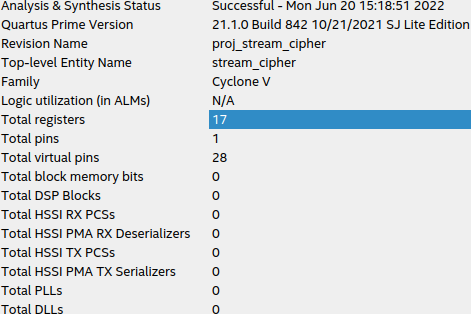
\includegraphics[width=.8\textwidth]{registers_synthesis}
    \caption{Analysis and synthesis summary}
    \label{fig:synthesizer_results_registers}
\end{figure}

The total number of registers reported in \cref{fig:summary}, however, is 23.
After checking the fitter result, it can be seen that this is due to routing optimizations, as reported by the Quartus Prime tool. In particular, as it can be seen in \cref{fig:fitter_duplicated_registers}, 6 registers, duplicated from \lstinline{cb[6:1]}, have been added to the final netlist.
\begin{figure}[!ht]
    \centering
    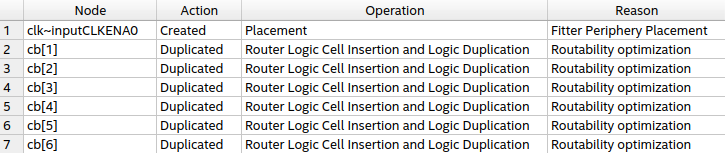
\includegraphics[width=.95\textwidth]{fitter_duplicated_registers}
    \caption{Fitter netlist optimization summary}
    \label{fig:fitter_duplicated_registers}
\end{figure}

